%%\documentclass[a4paper,12pt,oneside]{llncs}
\documentclass[12pt,letterpaper]{article}
\usepackage[right=2cm,left=3cm,top=2cm,bottom=2cm,headsep=0cm]{geometry}

%%%%%%%%%%%%%%%%%%%%%%%%%%%%%%%%%%%%%%%%%%%%%%%%%%%%%%%%%%%
%% Juego de caracteres usado en el archivo fuente: UTF-8
\usepackage{ucs}
\usepackage[utf8x]{inputenc}

%%%%%%%%%%%%%%%%%%%%%%%%%%%%%%%%%%%%%%%%%%%%%%%%%%%%%%%%%%%
%% Juego de caracteres usado en la salida dvi
%% Otra posibilidad: \usepackage{t1enc}
\usepackage[T1]{fontenc}

%%%%%%%%%%%%%%%%%%%%%%%%%%%%%%%%%%%%%%%%%%%%%%%%%%%%%%%%%%%
%% Ajusta maergenes para a4
%\usepackage{a4wide}

%%%%%%%%%%%%%%%%%%%%%%%%%%%%%%%%%%%%%%%%%%%%%%%%%%%%%%%%%%%
%% Uso fuente postscript times, para que los ps y pdf queden y pequeños...
\usepackage{times}

%%%%%%%%%%%%%%%%%%%%%%%%%%%%%%%%%%%%%%%%%%%%%%%%%%%%%%%%%%%
%% Posibilidad de hipertexto (especialmente en pdf)
%\usepackage{hyperref}
\usepackage[bookmarks = true, colorlinks=true, linkcolor = black, citecolor = black, menucolor = black, urlcolor = black]{hyperref}

%%%%%%%%%%%%%%%%%%%%%%%%%%%%%%%%%%%%%%%%%%%%%%%%%%%%%%%%%%%
%% Graficos 
\usepackage{graphics,graphicx}

%%%%%%%%%%%%%%%%%%%%%%%%%%%%%%%%%%%%%%%%%%%%%%%%%%%%%%%%%%%
%% Ciertos caracteres "raros"...
\usepackage{latexsym}

%%%%%%%%%%%%%%%%%%%%%%%%%%%%%%%%%%%%%%%%%%%%%%%%%%%%%%%%%%%
%% Matematicas aun más fuertes (american math dociety)
\usepackage{amsmath}

%%%%%%%%%%%%%%%%%%%%%%%%%%%%%%%%%%%%%%%%%%%%%%%%%%%%%%%%%%%
\usepackage{multirow} % para las tablas
\usepackage[spanish,es-tabla]{babel}

%%%%%%%%%%%%%%%%%%%%%%%%%%%%%%%%%%%%%%%%%%%%%%%%%%%%%%%%%%%
%% Fuentes matematicas lo mas compatibles posibles con postscript (times)
%% (Esto no funciona para todos los simbolos pero reduce mucho el tamaño del
%% pdf si hay muchas matamaticas....
\usepackage{mathptm}

%%% VARIOS:
%\usepackage{slashbox}
\usepackage{verbatim}
\usepackage{array}
\usepackage{listings}
\usepackage{multirow}

%% MARCA DE AGUA
%% Este package de "draft copy" NO funciona con pdflatex
%%\usepackage{draftcopy}
%% Este package de "draft copy" SI funciona con pdflatex
%%%\usepackage{pdfdraftcopy}
%%%%%%%%%%%%%%%%%%%%%%%%%%%%%%%%%%%%%%%%%%%%%%%%%%%%%%%%%%%
%% Indenteacion en español...
\usepackage[spanish]{babel}

\usepackage{listings}
% Para escribir código en C
% \begin{lstlisting}[language=C]
% #include <stdio.h>
% int main(int argc, char* argv[]) {
% puts("Hola mundo!");
% }
% \end{lstlisting}


\title{Análisis}
\author{Jesús Rodríguez Heras}

\begin{document}
	
	\maketitle
	\begin{abstract} %Poner esto en todas las prácticas de PCTR
		\begin{center}
			Desarrollo de la tabla con las conclusiones de usar varios hilos en la resolución de los problemas 1 y 2 de la práctica 4.
		\end{center}
	\end{abstract}
	\thispagestyle{empty}
	\newpage
	
	\tableofcontents
	\newpage
	
	%%\listoftables
	%%\newpage
	
	%%\listoffigures
	%%\newpage
	
	%%%% REAL WORK BEGINS HERE:
	
	%%Configuracion del paquete listings
	\lstset{language=bash, numbers=left, numberstyle=\tiny, numbersep=10pt, firstnumber=1, stepnumber=1, basicstyle=\small\ttfamily, tabsize=1, extendedchars=true, inputencoding=latin1}

\section{\texttt{matVector.java}}

Para las pruebas realizadas, hemos considerado una matriz cuadrada con el mismo número de columnas que elementos tiene el vector por el cual se multiplica dicha matriz.
\begin{center}
	\begin{table}[htbp]
		\begin{center}
			\begin{tabular}{|c|c|c|}
				\hline
				\textbf{Elementos} & \textbf{\% CPU} & \textbf{Tiempo (s)}  \\
				\hline 
				$500$ & 13 & 0.014\\ \hline	
				$1000$ & 17 & 0.011\\ \hline
				$1500$ & 19 & 0.013\\ \hline
				$2000$ & 21 & 0.015\\ \hline
				$2500$ & 31 & 0.016\\ \hline
				$3000$ & 32 & 0.021\\ \hline
				$3500$ & 38 & 0.024\\ \hline
				$4000$ & 47 & 0.026\\ \hline
				$4500$ & 58 & 0.034\\ \hline
				$5000$ & 64 & 0.04\\ \hline			
			\end{tabular}
			\caption{Valores de matVector.}
			\label{tabla:Valores de matVector}
		\end{center}
	\end{table}
\end{center}
\begin{figure}[h]
	\begin{center}
		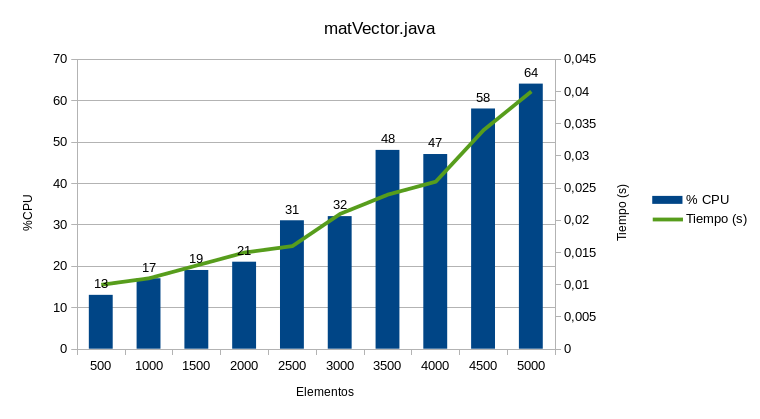
\includegraphics[scale=0.8]{matVector.png}
		\caption{Gráfica de matVector.}
		\label{fig: matVector}
	\end{center}
\end{figure}

\newpage
\section{\texttt{matVectorConcurrente.java}}

Para las pruebas realizadas, hemos utilizado una matriz cuadrada con el mismo número de columnas que elementos tiene el vector por el cual se multiplica dicha matriz. Este algoritmo crea un hilo por cada elemento del vector resultante.
\begin{center}
	\begin{table}[htbp]
		\begin{center}
			\begin{tabular}{|c|c|c|}
				\hline
				\textbf{Elementos} & \textbf{\% CPU} & \textbf{Tiempo (s)}  \\
				\hline 
				$500$ & 18 & 0.093\\ \hline	
				$1000$ & 20 & 0.096\\ \hline
				$1500$ & 24 & 0.133\\ \hline
				$2000$ & 23 & 0.186\\ \hline
				$2500$ & 22 & 0.216\\ \hline
				$3000$ & 36 & 0.232\\ \hline
				$3500$ & 46 & 0.276\\ \hline
				$4000$ & 47 & 0.269\\ \hline
				$4500$ & 49 & 0.32\\ \hline
				$5000$ & 43 & 0.356\\ \hline		
			\end{tabular}
			\caption{Valores de matVectorConcurrente.}
			\label{tabla:Valores de matVectorConcurrente}
		\end{center}
	\end{table}
\end{center}
\begin{figure}[h]
	\begin{center}
		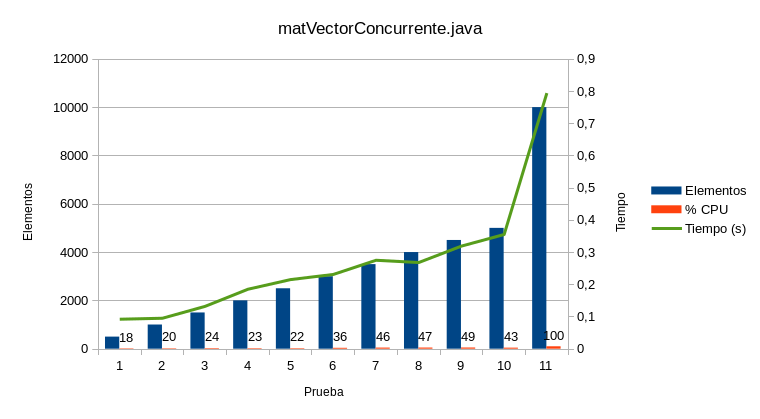
\includegraphics[scale=0.8]{matVectorConcurrente.png}
		\caption{Gráfica de matVectorConcurrente.}
		\label{fig: matVectorConcurrente}
	\end{center}	
\end{figure}

\newpage
\section{\texttt{prodMat.java}}

Para las pruebas realizadas hemos usado matrices cuadradas.
\begin{center}
	\begin{table}[htbp]
		\begin{center}
			\begin{tabular}{|c|c|c|}
				\hline
				\textbf{Elementos} & \textbf{\% CPU} & \textbf{Tiempo (s)}  \\
				\hline 
				$500$ & 36 & 0.395\\ \hline	
				$1000$ & 100 & 15.982\\ \hline
				$1500$ & 100 & 63.443\\ \hline
				$2000$ & 100 & 159.822\\ \hline
				$2500$ & 100 & 323.924\\ \hline
			\end{tabular}
			\caption{Valores de prodMat.}
			\label{tabla:Valores de prodMat}
		\end{center}
	\end{table}
\end{center}

Viendo como va evolucionando la tabla, poner más valores es innecesario, ya que sería inviable para valores más altos.

\begin{figure}[h]
	\begin{center}
		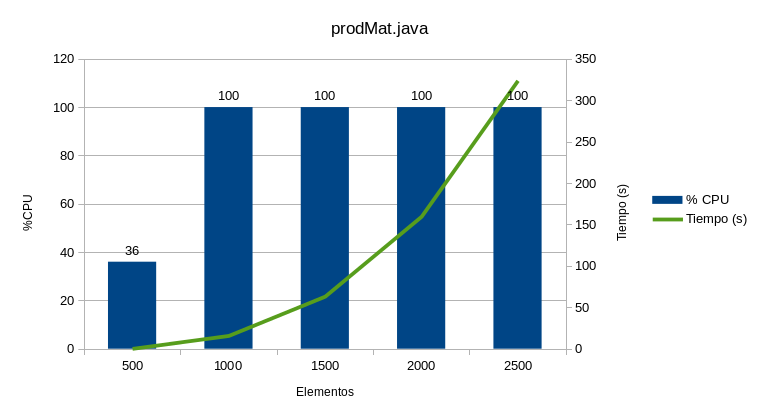
\includegraphics[scale=0.8]{prodMat.png}
		\caption{Gráfica de prodMat.}
		\label{fig: prodMat}
	\end{center}	
\end{figure}


\newpage
\section{\texttt{prodMatConcurrente.java}}

Para las pruebas realizadas, hemos usado matrices cuadradas. Este algoritmo crea un hilo por cada fila de la matriz resultante.
\begin{center}
	\begin{table}[htbp]
		\begin{center}
			\begin{tabular}{|c|c|c|}
				\hline
				\textbf{Elementos} & \textbf{\% CPU} & \textbf{Tiempo (s)}  \\
				\hline 
				$25$ & 24 & 0.083\\ \hline
				$50$ & 17 & 0.211\\ \hline
				$100$ & 34 & 0.738\\ \hline	
				$200$ & 53 & 3.609 \\ \hline 
				$300$ & 66 & 13.348 \\ \hline 
				$400$ & 69 & 37.195 \\ \hline 
				$500$ & 74 & 114.118\\ \hline
			\end{tabular}
			\caption{Valores de prodMatConcurrente.}
			\label{tabla:Valores de prodMatConcurrente}
		\end{center}
	\end{table}
\end{center}

Debido al uso de excesivos hilos, si aumentamos el numero de filas/columnas a más de 500, el programa tarda mucho en ejecutarse y con la batería de pruebas mostrada se ve el crecimiento que tiene.
\begin{figure}[h]
	\begin{center}
		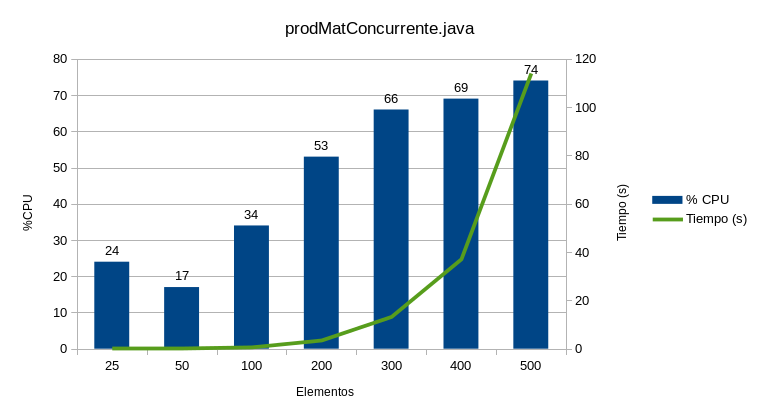
\includegraphics[scale=0.8]{prodMatConcurrente.png}
		\caption{Gráfica de prodMatConcurrente.}
		\label{fig: Gráfica de prodMatConcurrente}
	\end{center}	
\end{figure}

\newpage
\section{Impresiones recabadas}

Viendo los resultado obtenidos en las pruebas de los diversos algoritmos, podemos deducir que el hecho de crear más hilos, no nos determina la velocidad con la que se ejecutará un programa.

Esto es así, debido a que la creación de hilos, nos genera un coste de tiempo y de memoria que puede ser crucial en otros aspectos.

El ejemplo más claro lo obtenemos entre los algoritmos \texttt{prodMat.java} y\\ \texttt{prodMatConcurrente.java} donde, con dos matrices de $500x500$ elementos, en el primero de ellos (secuencial) tardamos 0.395 segundos, mientras que en el segundo (concurrente) tardamos 114.118 segundos.

\end{document}